\documentclass[man]{apa6}
\usepackage{lmodern}
\usepackage{amssymb,amsmath}
\usepackage{ifxetex,ifluatex}
\usepackage{fixltx2e} % provides \textsubscript
\ifnum 0\ifxetex 1\fi\ifluatex 1\fi=0 % if pdftex
  \usepackage[T1]{fontenc}
  \usepackage[utf8]{inputenc}
\else % if luatex or xelatex
  \ifxetex
    \usepackage{mathspec}
  \else
    \usepackage{fontspec}
  \fi
  \defaultfontfeatures{Ligatures=TeX,Scale=MatchLowercase}
\fi
% use upquote if available, for straight quotes in verbatim environments
\IfFileExists{upquote.sty}{\usepackage{upquote}}{}
% use microtype if available
\IfFileExists{microtype.sty}{%
\usepackage{microtype}
\UseMicrotypeSet[protrusion]{basicmath} % disable protrusion for tt fonts
}{}
\usepackage{hyperref}
\hypersetup{unicode=true,
            pdftitle={Does Music Convey Social Information to Infants?},
            pdfauthor={Mehr, Song~\& Spelke},
            pdfkeywords={keywords},
            pdfborder={0 0 0},
            breaklinks=true}
\urlstyle{same}  % don't use monospace font for urls
\usepackage{graphicx,grffile}
\makeatletter
\def\maxwidth{\ifdim\Gin@nat@width>\linewidth\linewidth\else\Gin@nat@width\fi}
\def\maxheight{\ifdim\Gin@nat@height>\textheight\textheight\else\Gin@nat@height\fi}
\makeatother
% Scale images if necessary, so that they will not overflow the page
% margins by default, and it is still possible to overwrite the defaults
% using explicit options in \includegraphics[width, height, ...]{}
\setkeys{Gin}{width=\maxwidth,height=\maxheight,keepaspectratio}
\IfFileExists{parskip.sty}{%
\usepackage{parskip}
}{% else
\setlength{\parindent}{0pt}
\setlength{\parskip}{6pt plus 2pt minus 1pt}
}
\setlength{\emergencystretch}{3em}  % prevent overfull lines
\providecommand{\tightlist}{%
  \setlength{\itemsep}{0pt}\setlength{\parskip}{0pt}}
\setcounter{secnumdepth}{0}
% Redefines (sub)paragraphs to behave more like sections
\ifx\paragraph\undefined\else
\let\oldparagraph\paragraph
\renewcommand{\paragraph}[1]{\oldparagraph{#1}\mbox{}}
\fi
\ifx\subparagraph\undefined\else
\let\oldsubparagraph\subparagraph
\renewcommand{\subparagraph}[1]{\oldsubparagraph{#1}\mbox{}}
\fi

%%% Use protect on footnotes to avoid problems with footnotes in titles
\let\rmarkdownfootnote\footnote%
\def\footnote{\protect\rmarkdownfootnote}


  \title{Does Music Convey Social Information to Infants?}
    \author{Mehr, Song\textsuperscript{1}~\& Spelke\textsuperscript{1,2}}
    \date{}
  
\shorttitle{Title}
\affiliation{
\vspace{0.5cm}
\textsuperscript{1} Wilhelm-Wundt-University\\\textsuperscript{2} Konstanz Business School}
\keywords{keywords\newline\indent Word count: X}
\usepackage{csquotes}
\usepackage{upgreek}
\captionsetup{font=singlespacing,justification=justified}

\usepackage{longtable}
\usepackage{lscape}
\usepackage{multirow}
\usepackage{tabularx}
\usepackage[flushleft]{threeparttable}
\usepackage{threeparttablex}

\newenvironment{lltable}{\begin{landscape}\begin{center}\begin{ThreePartTable}}{\end{ThreePartTable}\end{center}\end{landscape}}

\makeatletter
\newcommand\LastLTentrywidth{1em}
\newlength\longtablewidth
\setlength{\longtablewidth}{1in}
\newcommand{\getlongtablewidth}{\begingroup \ifcsname LT@\roman{LT@tables}\endcsname \global\longtablewidth=0pt \renewcommand{\LT@entry}[2]{\global\advance\longtablewidth by ##2\relax\gdef\LastLTentrywidth{##2}}\@nameuse{LT@\roman{LT@tables}} \fi \endgroup}


\DeclareDelayedFloatFlavor{ThreePartTable}{table}
\DeclareDelayedFloatFlavor{lltable}{table}
\DeclareDelayedFloatFlavor*{longtable}{table}
\makeatletter
\renewcommand{\efloat@iwrite}[1]{\immediate\expandafter\protected@write\csname efloat@post#1\endcsname{}}
\makeatother
\usepackage{lineno}

\linenumbers

\authornote{Add complete departmental affiliations for each
author here. Each new line herein must be indented, like this line.

Enter author note here.

Correspondence concerning this article should be addressed to Mehr,
Song, Postal address. E-mail:
\href{mailto:my@email.com}{\nolinkurl{my@email.com}}}

\abstract{
One or two sentences providing a \textbf{basic introduction} to the
field, comprehensible to a scientist in any discipline. Five month old
infants were exposed to one of two novel songs containing different
melodies with lyrics and rhythms being the same. Infants either heard
the songs through a toy in which their parent's voice was recorded or
was sung live by a friendly unfamiliar person initially and later
through video recording. Infant's selective attention was tested by
having them listen to two presentations of either familiar or unfamiliar
songs. Infants payed attention to the familiar song, sung by their
parent in the past. No infant preference was observed between the toy
onto which parent's voice was recorde or a video recording of an
unfamiliar person, briefly met by an infant initially. Infants in the
later two conditions retained the memory of the melody for longer than 8
months. These findings suggest that songs performed by parents at home
convey social meaning to a child.

Two to three sentences of \textbf{more detailed background},
comprehensible to scientists in related disciplines.

One sentence clearly stating the \textbf{general problem} being
addressed by this particular study.

One sentence summarizing the main result (with the words ``\textbf{here
we show}'' or their equivalent).

Two or three sentences explaining what the \textbf{main result} reveals
in direct comparison to what was thought to be the case previously, or
how the main result adds to previous knowledge.

One or two sentences to put the results into a more \textbf{general
context}.

Two or three sentences to provide a \textbf{broader perspective},
readily comprehensible to a scientist in any discipline.


}

\begin{document}
\maketitle

Introduction - Music is a universal phenomenon that captures our
imaginations throughout our lifetime, starting from early childhood.
Parents usually sing to their infants and children in a globally
recognizable style of singing.

\subsection{subheader}\label{subheader}

\section{Methods}\label{methods}

We report how we determined our sample size, all data exclusions (if
any), all manipulations, and all measures in the study.

\subsection{Participants}\label{participants}

\subsection{Material}\label{material}

\subsection{Procedure}\label{procedure}

\subsection{Data analysis}\label{data-analysis}

We used R (Version 3.5.2; R Core Team, 2018) and the R-packages
\emph{data.table} (Version 1.12.0; Dowle \& Srinivasan, 2019),
\emph{dplyr} (Version 0.8.0.1; Wickham, François, Henry, \& Müller,
2019), \emph{papaja} (Version 0.1.0.9842; Aust \& Barth, 2018),
\emph{pwr} (Version 1.2.2; Champely, 2018), and \emph{summarytools}
(Version 0.9.2; Comtois, 2019) for all our analyses.

\begin{verbatim}
## Warning: package 'summarytools' was built under R version 3.5.3
\end{verbatim}

\begin{figure}
\centering
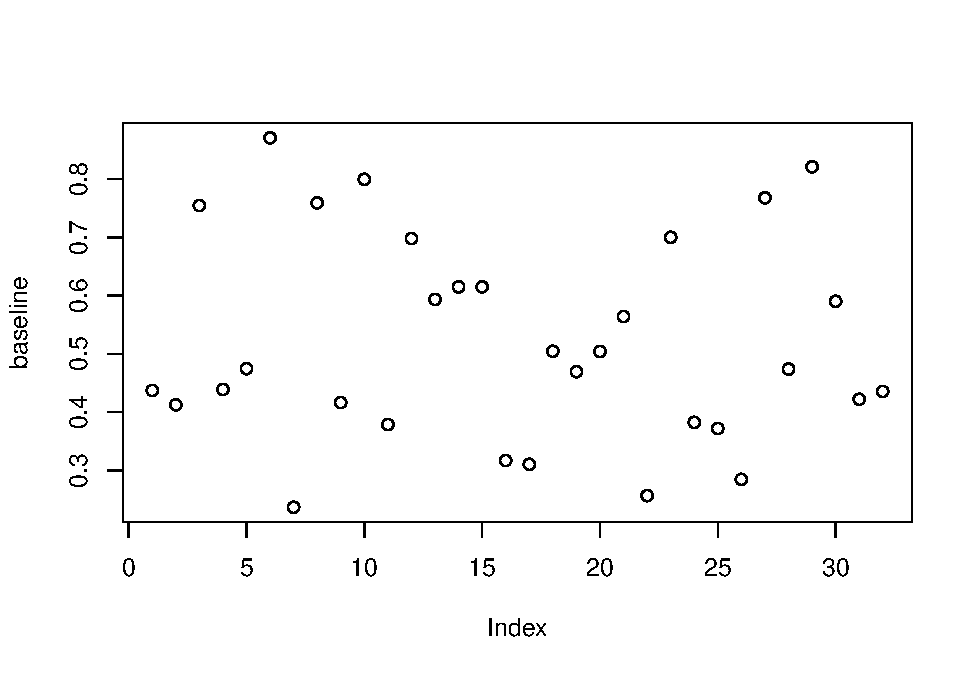
\includegraphics{test_papaja_files/figure-latex/unnamed-chunk-5-1.pdf}
\caption{}
\end{figure}

\section{Results}\label{results}

lets say we want to make a figure if we wanted to find power

\begin{verbatim}
## Warning: package 'pwr' was built under R version 3.5.3
\end{verbatim}

\begin{verbatim}
## 
##      Two-sample t test power calculation 
## 
##               n = 44
##               d = 0.8
##       sig.level = 0.05
##           power = 0.9599534
##     alternative = two.sided
## 
## NOTE: n is number in *each* group
\end{verbatim}

\begin{figure}
\centering
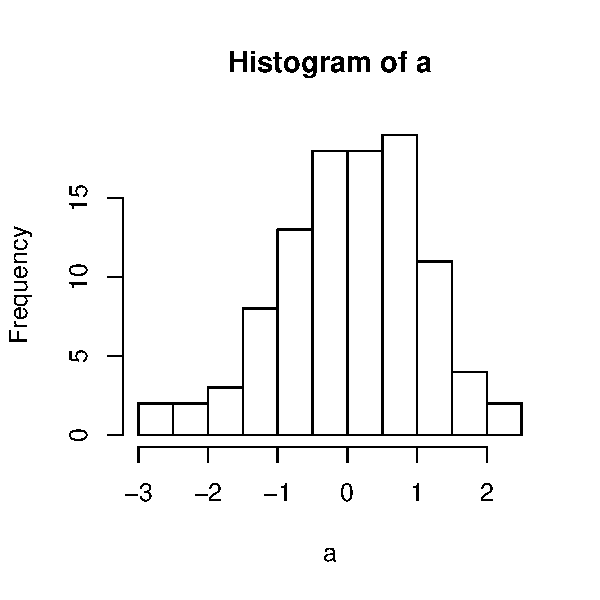
\includegraphics{test_papaja_files/figure-latex/myfig-1.pdf}
\caption{\label{fig:myfig}this is a histograpm}
\end{figure}

\begin{figure}
\centering
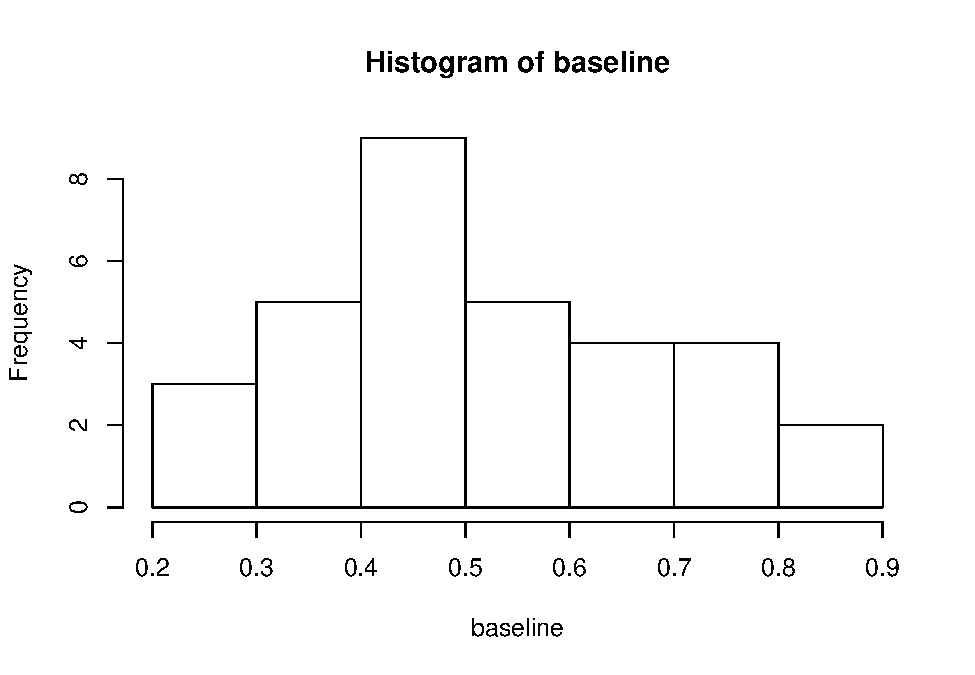
\includegraphics{test_papaja_files/figure-latex/unnamed-chunk-8-1.pdf}
\caption{}
\end{figure}

\begin{verbatim}
## [1] 0.5210967
\end{verbatim}

\begin{verbatim}
## [1] 0.1769651
\end{verbatim}

\begin{verbatim}
## [1] 0.1769651
\end{verbatim}

\section{Discussion}\label{discussion}

\newpage

\section{References}\label{references}

Mehr, S. A., Song. L. A., \& Spelke, E. S. (2016). For 5-month-old
infants, melodies are social. Psychological Science, 27, 486-501 Crump,
McDonnell, and Gureckis (2013) did some experiments

\begingroup
\setlength{\parindent}{-0.5in} \setlength{\leftskip}{0.5in}

\hypertarget{refs}{}
\hypertarget{ref-R-papaja}{}
Aust, F., \& Barth, M. (2018). \emph{papaja: Create APA manuscripts with
R Markdown}. Retrieved from \url{https://github.com/crsh/papaja}

\hypertarget{ref-R-pwr}{}
Champely, S. (2018). \emph{Pwr: Basic functions for power analysis}.
Retrieved from \url{https://CRAN.R-project.org/package=pwr}

\hypertarget{ref-R-summarytools}{}
Comtois, D. (2019). \emph{Summarytools: Tools to quickly and neatly
summarize data}. Retrieved from
\url{https://CRAN.R-project.org/package=summarytools}

\hypertarget{ref-crump2013evaluating}{}
Crump, M. J., McDonnell, J. V., \& Gureckis, T. M. (2013). Evaluating
amazon's mechanical turk as a tool for experimental behavioral research.
\emph{PloS One}, \emph{8}(3), e57410.

\hypertarget{ref-R-data.table}{}
Dowle, M., \& Srinivasan, A. (2019). \emph{Data.table: Extension of
`data.frame`}. Retrieved from
\url{https://CRAN.R-project.org/package=data.table}

\hypertarget{ref-R-base}{}
R Core Team. (2018). \emph{R: A language and environment for statistical
computing}. Vienna, Austria: R Foundation for Statistical Computing.
Retrieved from \url{https://www.R-project.org/}

\hypertarget{ref-R-dplyr}{}
Wickham, H., François, R., Henry, L., \& Müller, K. (2019). \emph{Dplyr:
A grammar of data manipulation}. Retrieved from
\url{https://CRAN.R-project.org/package=dplyr}

\endgroup


\end{document}
